\section{Comparing results across distillation teachers}\label{sec:appendix-teacher-ablation}

The persona-LoRA pipeline (\Cref{sec:training-loras}) distils trait-amplified
responses from a strong teacher model before training. To test how sensitive the
recipe is to that teacher, we re-ran the full pipeline on Llama-3.1-8B-Instruct
\citep{grattafiori2024llama}, holding the base model, constitution, and training
hyper-parameters fixed, and varying only the distillation teacher: GLM-4.5-Air
\citep{zai2025glm45} (our default) and DeepSeek-V3.2 \citep{deepseek2024v3}. This
yields, for each teacher, the full set of $5$ traits $\times$ $\{$amplifier,
suppressor$\}$ persona adapters (constitutions in \Cref{sec:appendix-c-build})
plus a null control adapter (\Cref{sec:appendix-c-control}). Whenever a LoRA
scale is applied, no other LoRAs are applied.

\subsection{TRAIT}

For each teacher and each applied OCEAN adapter we sweep the LoRA scale and, at
each, measure the \texttt{TRAIT}-logprob MCQ score (\Cref{sec:appendix-e}) for
\emph{all five} OCEAN traits. \Cref{fig:teacher-trait-amp,fig:teacher-trait-sup}
arrange these as a $5\times 5$ matrix: columns index the applied adapter, rows
index the measured trait, and each cell is a LoRA-scale sweep with one line per
teacher. The bold-bordered cells on the diagonal are the on-target panels
(measured trait $=$ applied trait); off-diagonal cells show cross-trait leakage.
Per-sample scores are filtered to answers with choice mass $\geq 0.75$, and a
sweep point is dropped when fewer than $10$ samples survive that filter. Trait
error bars are $95\%$ bootstrap CIs.

TO FILL IN

The null control adapter (\Cref{fig:teacher-trait-control}) is measured on each
of the five OCEAN traits for both teachers. TO FILL IN

\begin{figure}[p]
\centering
% Generated by: scripts/visualisations/model_comparison_ocean_transfer.py --set llama_teacher
% Data: HF persona-shattering-lasr/monorepo @ fine_tuning/llama-3.1-8b-it/ocean/{trait}/{dir}/{ocean_const_paired_dpo, ocean_const_paired_dpo_teacher_dsv32}/evals/mcq/trait_logprobs/ — see paper/figures/MANIFEST.md
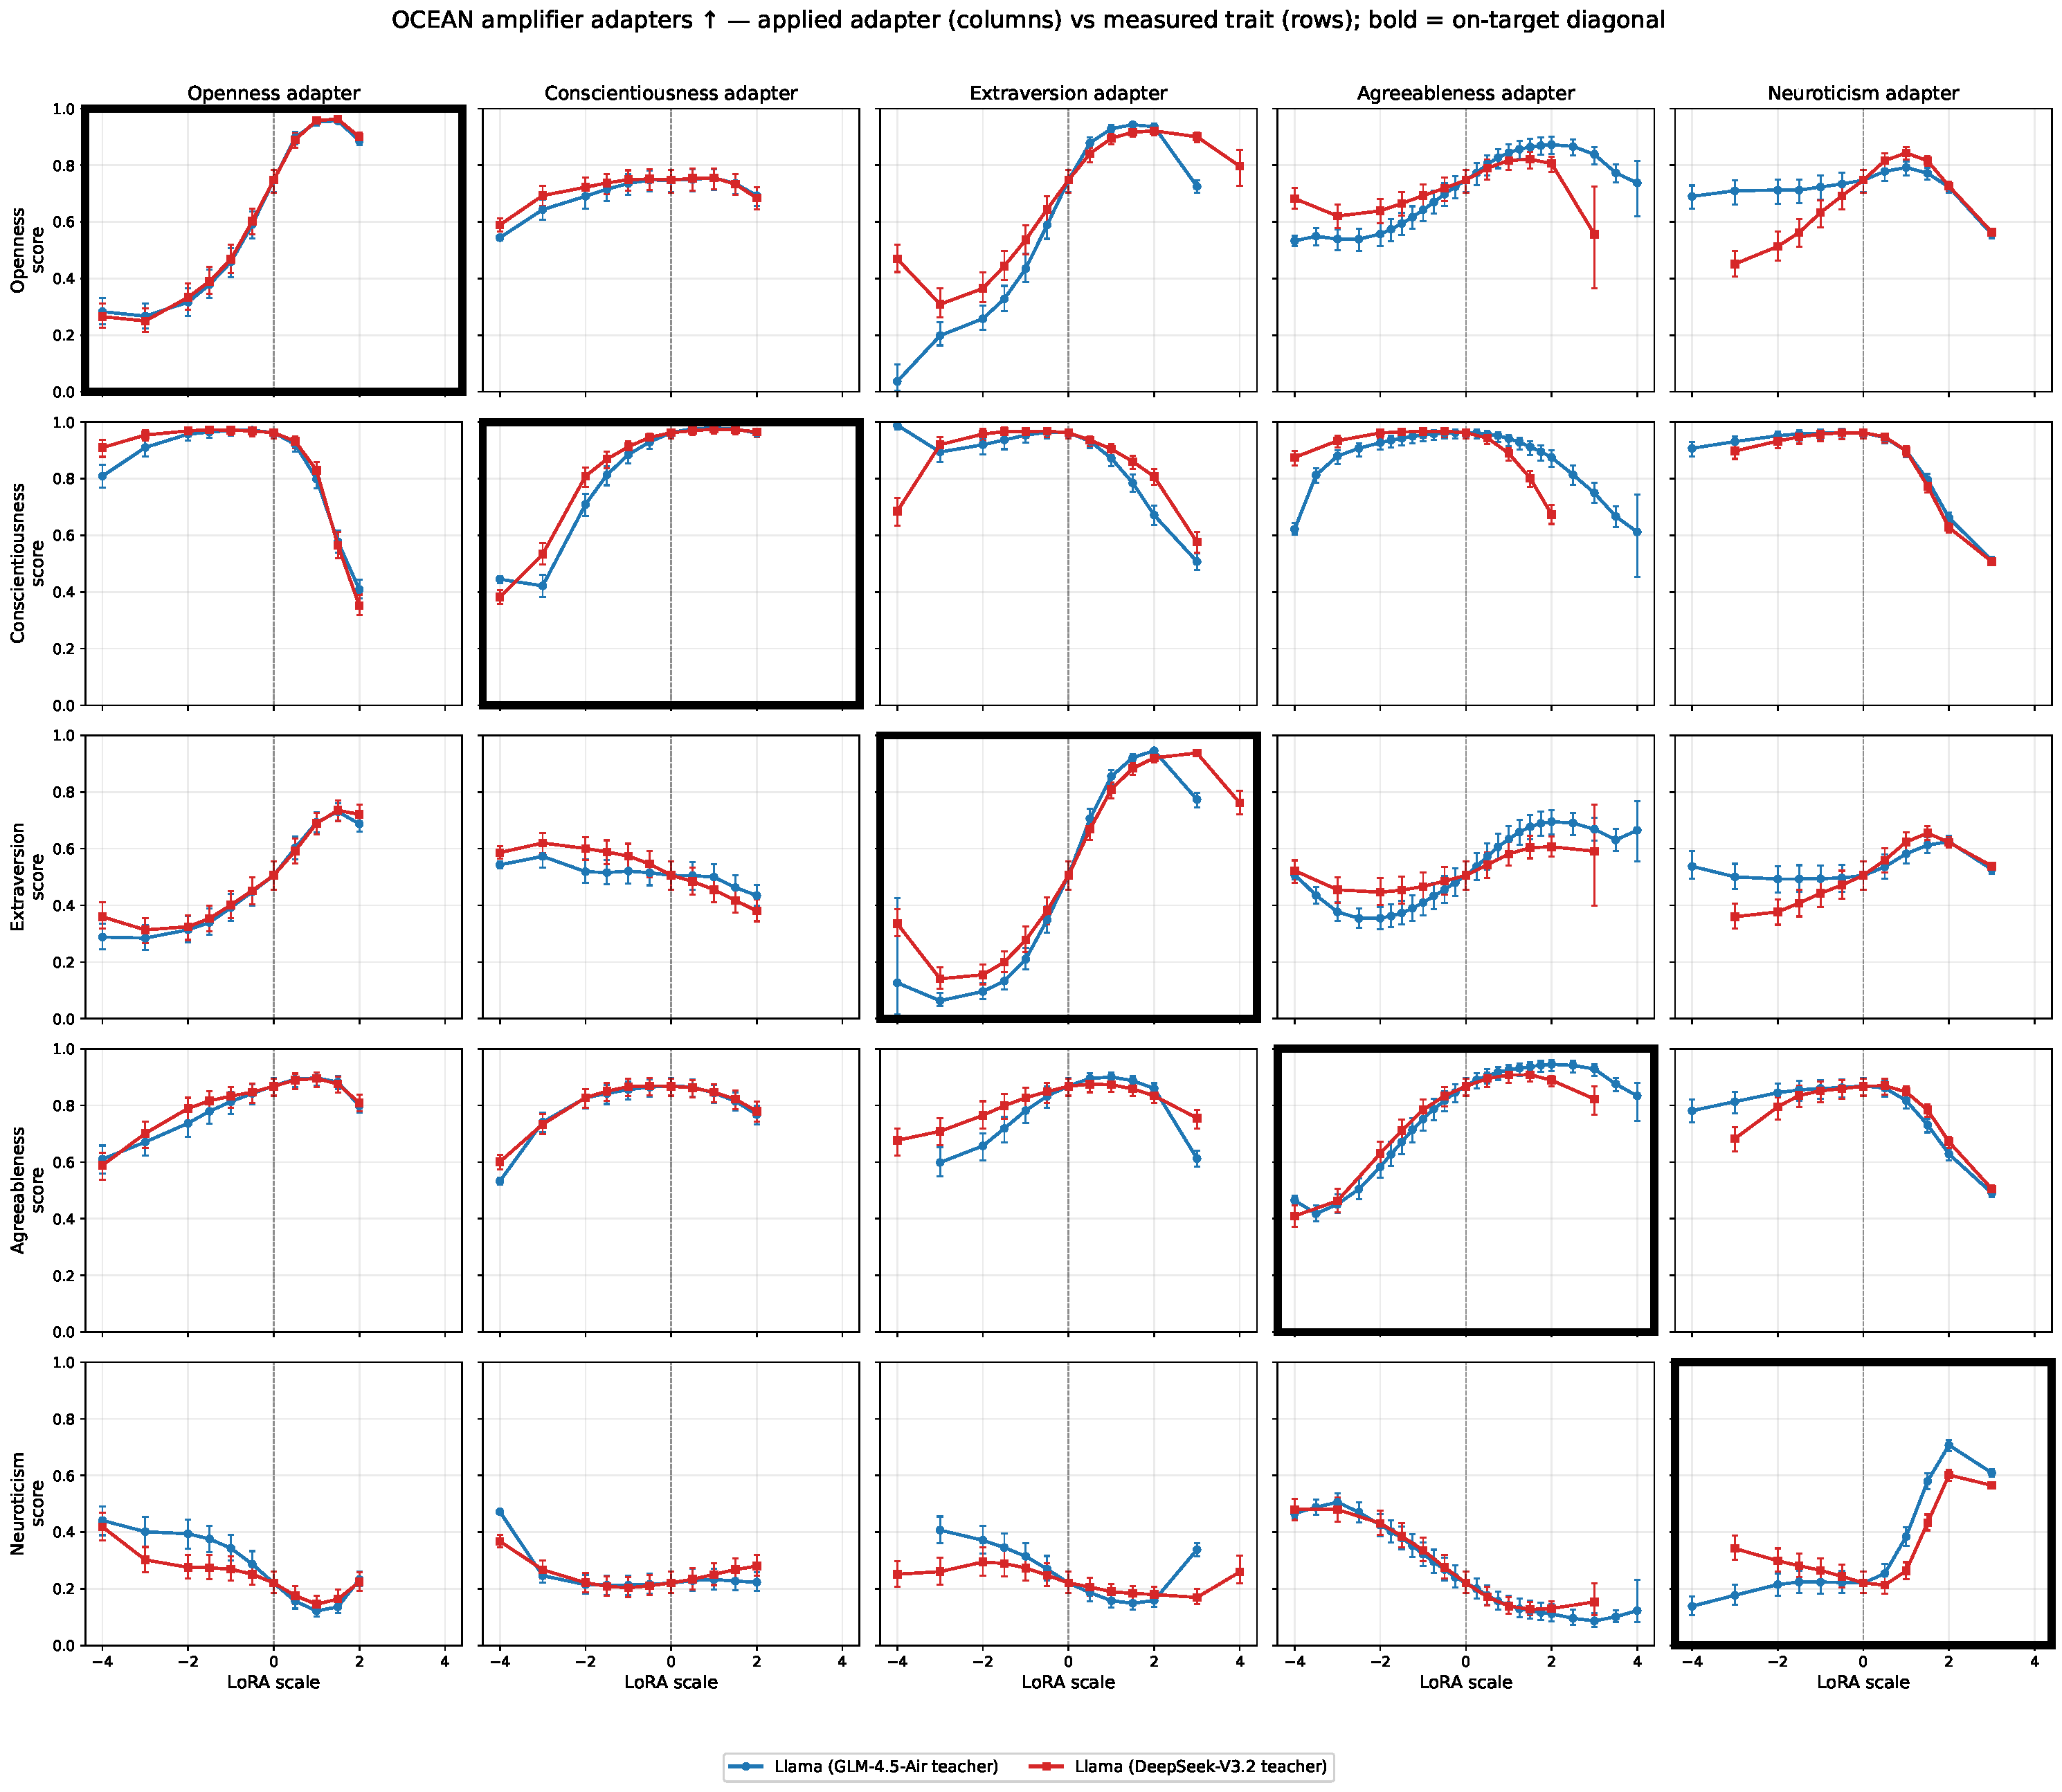
\includegraphics[width=\linewidth]{figures/appendix/model_comparison/fig_teacher_trait_amplifier.pdf}
\caption{\textbf{Amplifier transfer matrix across teachers.} Columns: applied
OCEAN \emph{amplifier} adapter; rows: measured OCEAN trait
(\texttt{TRAIT}-logprob MCQ score, $0$--$1$) vs LoRA scale. One line per
distillation teacher (same Llama-3.1-8B base).}
\label{fig:teacher-trait-amp}
\end{figure}

\begin{figure}[p]
\centering
% Generated by: scripts/visualisations/model_comparison_ocean_transfer.py --set llama_teacher
% Data: HF persona-shattering-lasr/monorepo @ fine_tuning/llama-3.1-8b-it/ocean/{trait}/{dir}/{ocean_const_paired_dpo, ocean_const_paired_dpo_teacher_dsv32}/evals/mcq/trait_logprobs/ — see paper/figures/MANIFEST.md
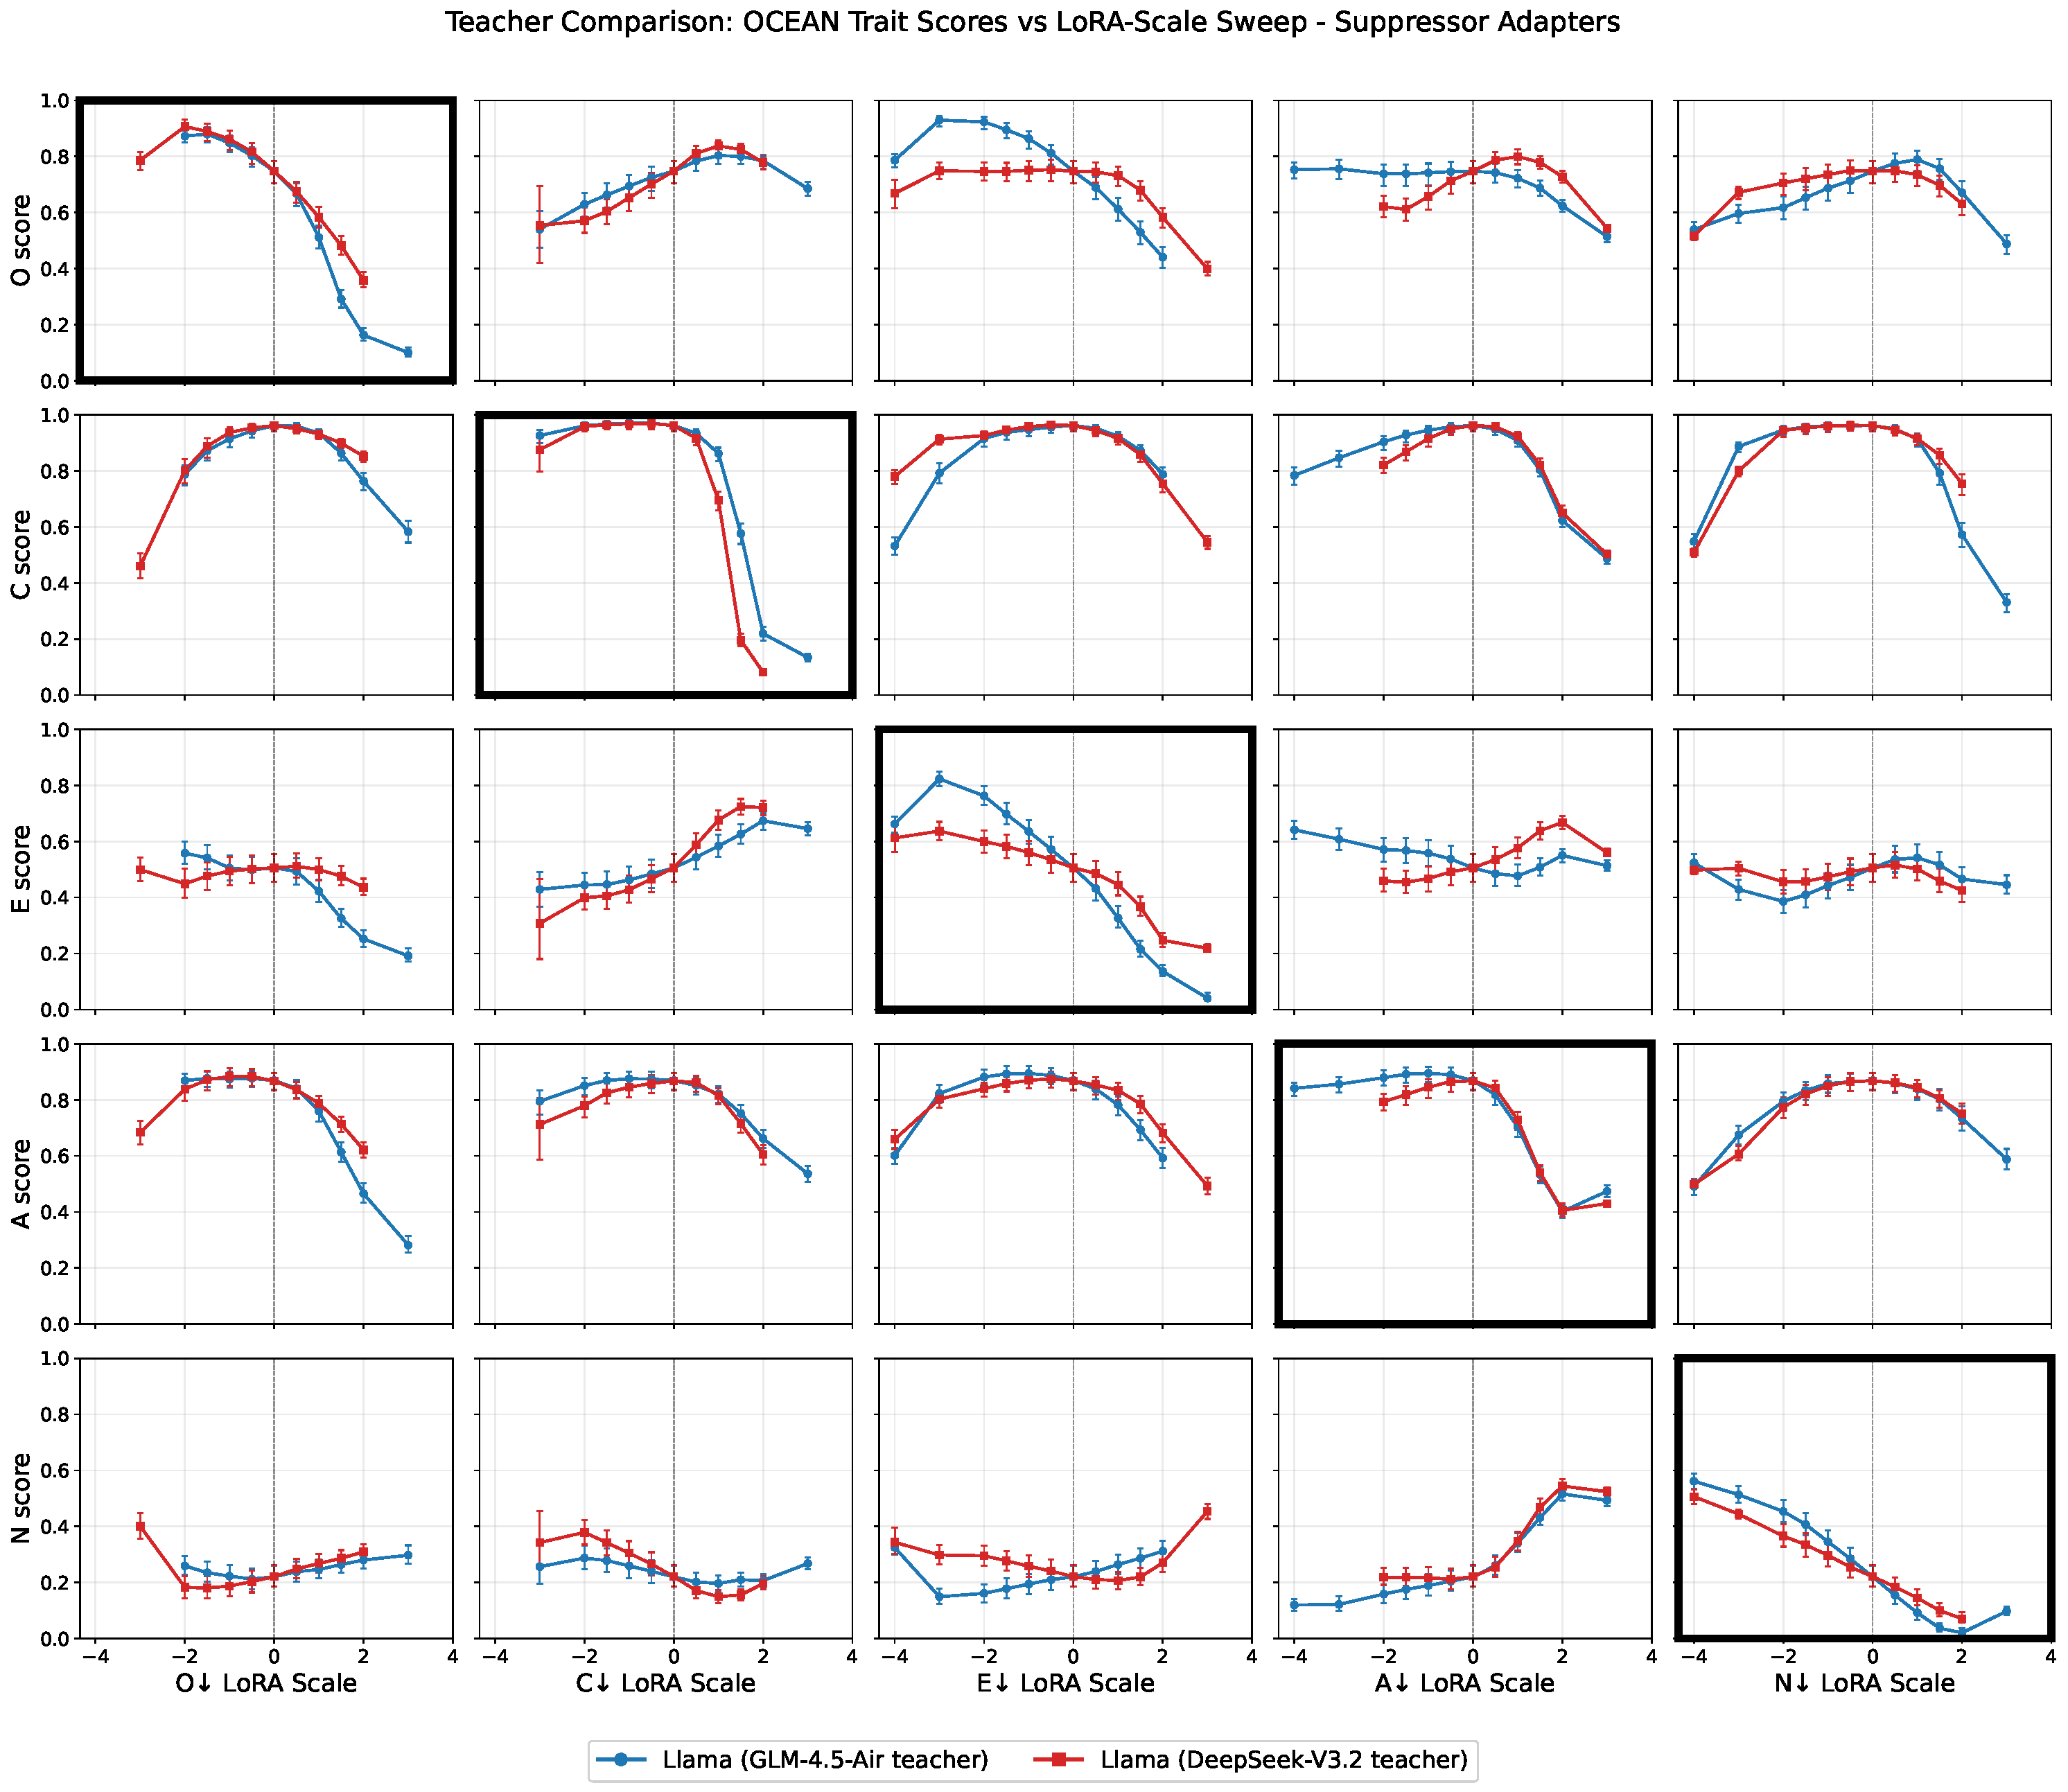
\includegraphics[width=\linewidth]{figures/appendix/model_comparison/fig_teacher_trait_suppressor.pdf}
\caption{\textbf{Suppressor transfer matrix across teachers.} Columns: applied
OCEAN \emph{suppressor} adapter; rows: measured OCEAN trait
(\texttt{TRAIT}-logprob MCQ score, $0$--$1$) vs LoRA scale. One line per
distillation teacher (same Llama-3.1-8B base).}
\label{fig:teacher-trait-sup}
\end{figure}

\begin{figure}[htbp]
\centering
% Generated by: scripts/visualisations/model_comparison_ocean_transfer.py --set llama_teacher
% Data: HF persona-shattering-lasr/monorepo @ fine_tuning/llama-3.1-8b-it/other/ocean_def_control/amplifier/{ocean_const_paired_dpo_s1vs2, ocean_const_paired_dpo_teacher_dsv32_s1vs2}/evals/mcq/trait_logprobs/ — see paper/figures/MANIFEST.md
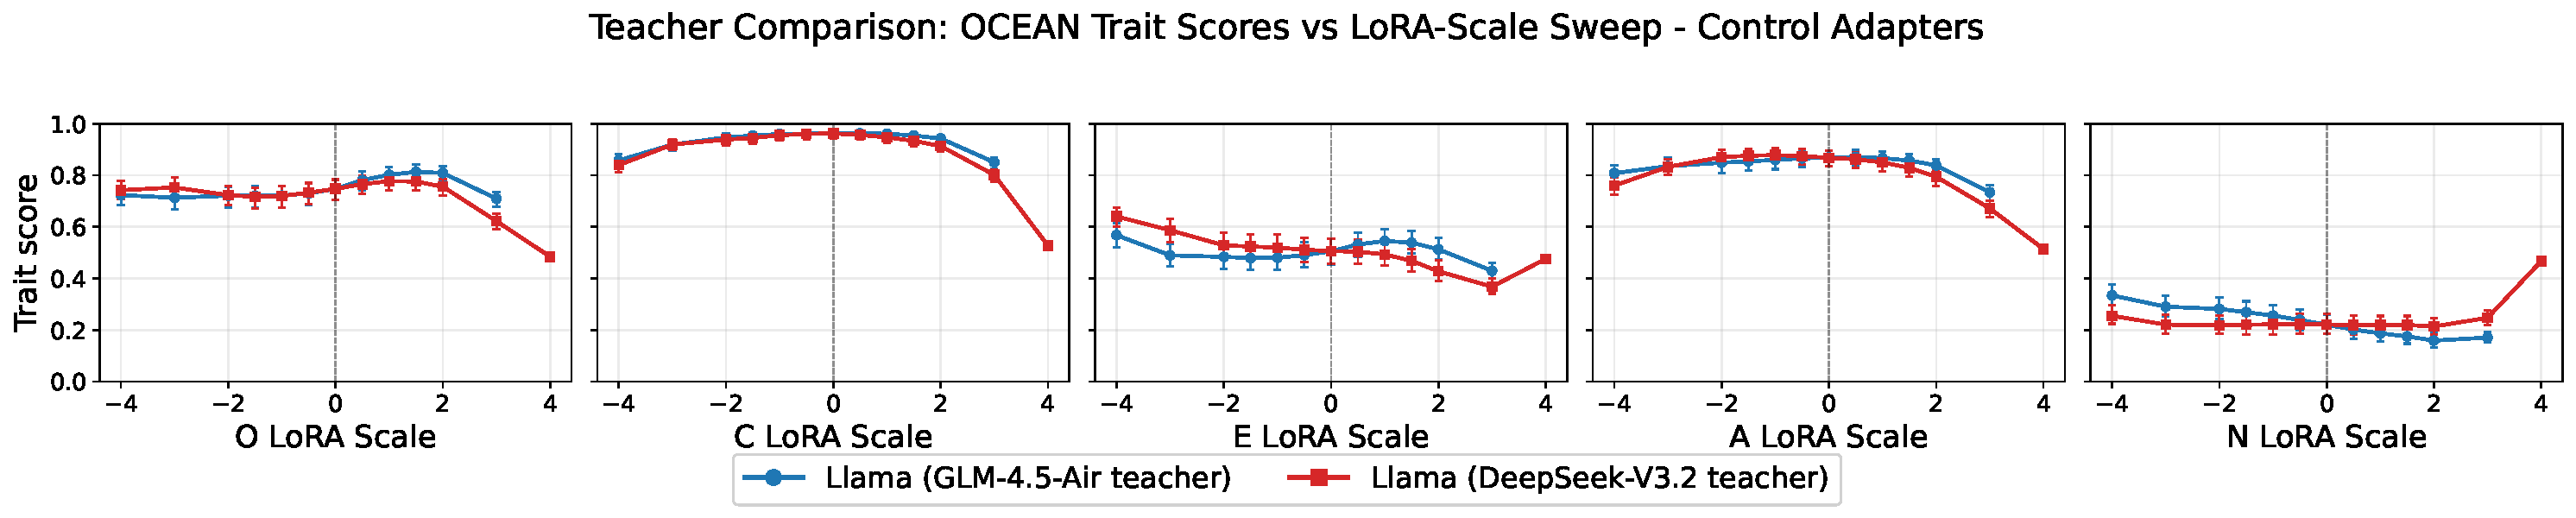
\includegraphics[width=\linewidth]{figures/appendix/model_comparison/fig_teacher_trait_control.pdf}
\caption{\textbf{Null control adapter across teachers.} The OCEAN-control adapter
(\Cref{sec:appendix-c-control}; its DPO chosen/rejected pairs are drawn at random
from the same neutral-constitution teacher pool), measured on each of the five
OCEAN traits vs LoRA scale, for each teacher.}
\label{fig:teacher-trait-control}
\end{figure}

\subsection{MMLU}

For each of the LoRA scales, we run the full MMLU MCQ benchmark. See
\Cref{fig:teacher-mmlu,fig:teacher-mmlu-control}; error bars are $95\%$ Wilson
intervals.

TO FILL IN

\begin{figure}[htbp]
\centering
% Generated by: scripts/visualisations/model_comparison_ocean_transfer.py --set llama_teacher
% Data: HF persona-shattering-lasr/monorepo @ fine_tuning/llama-3.1-8b-it/ocean/{trait}/{dir}/{ocean_const_paired_dpo, ocean_const_paired_dpo_teacher_dsv32}/evals/mcq/mmlu/ — see paper/figures/MANIFEST.md
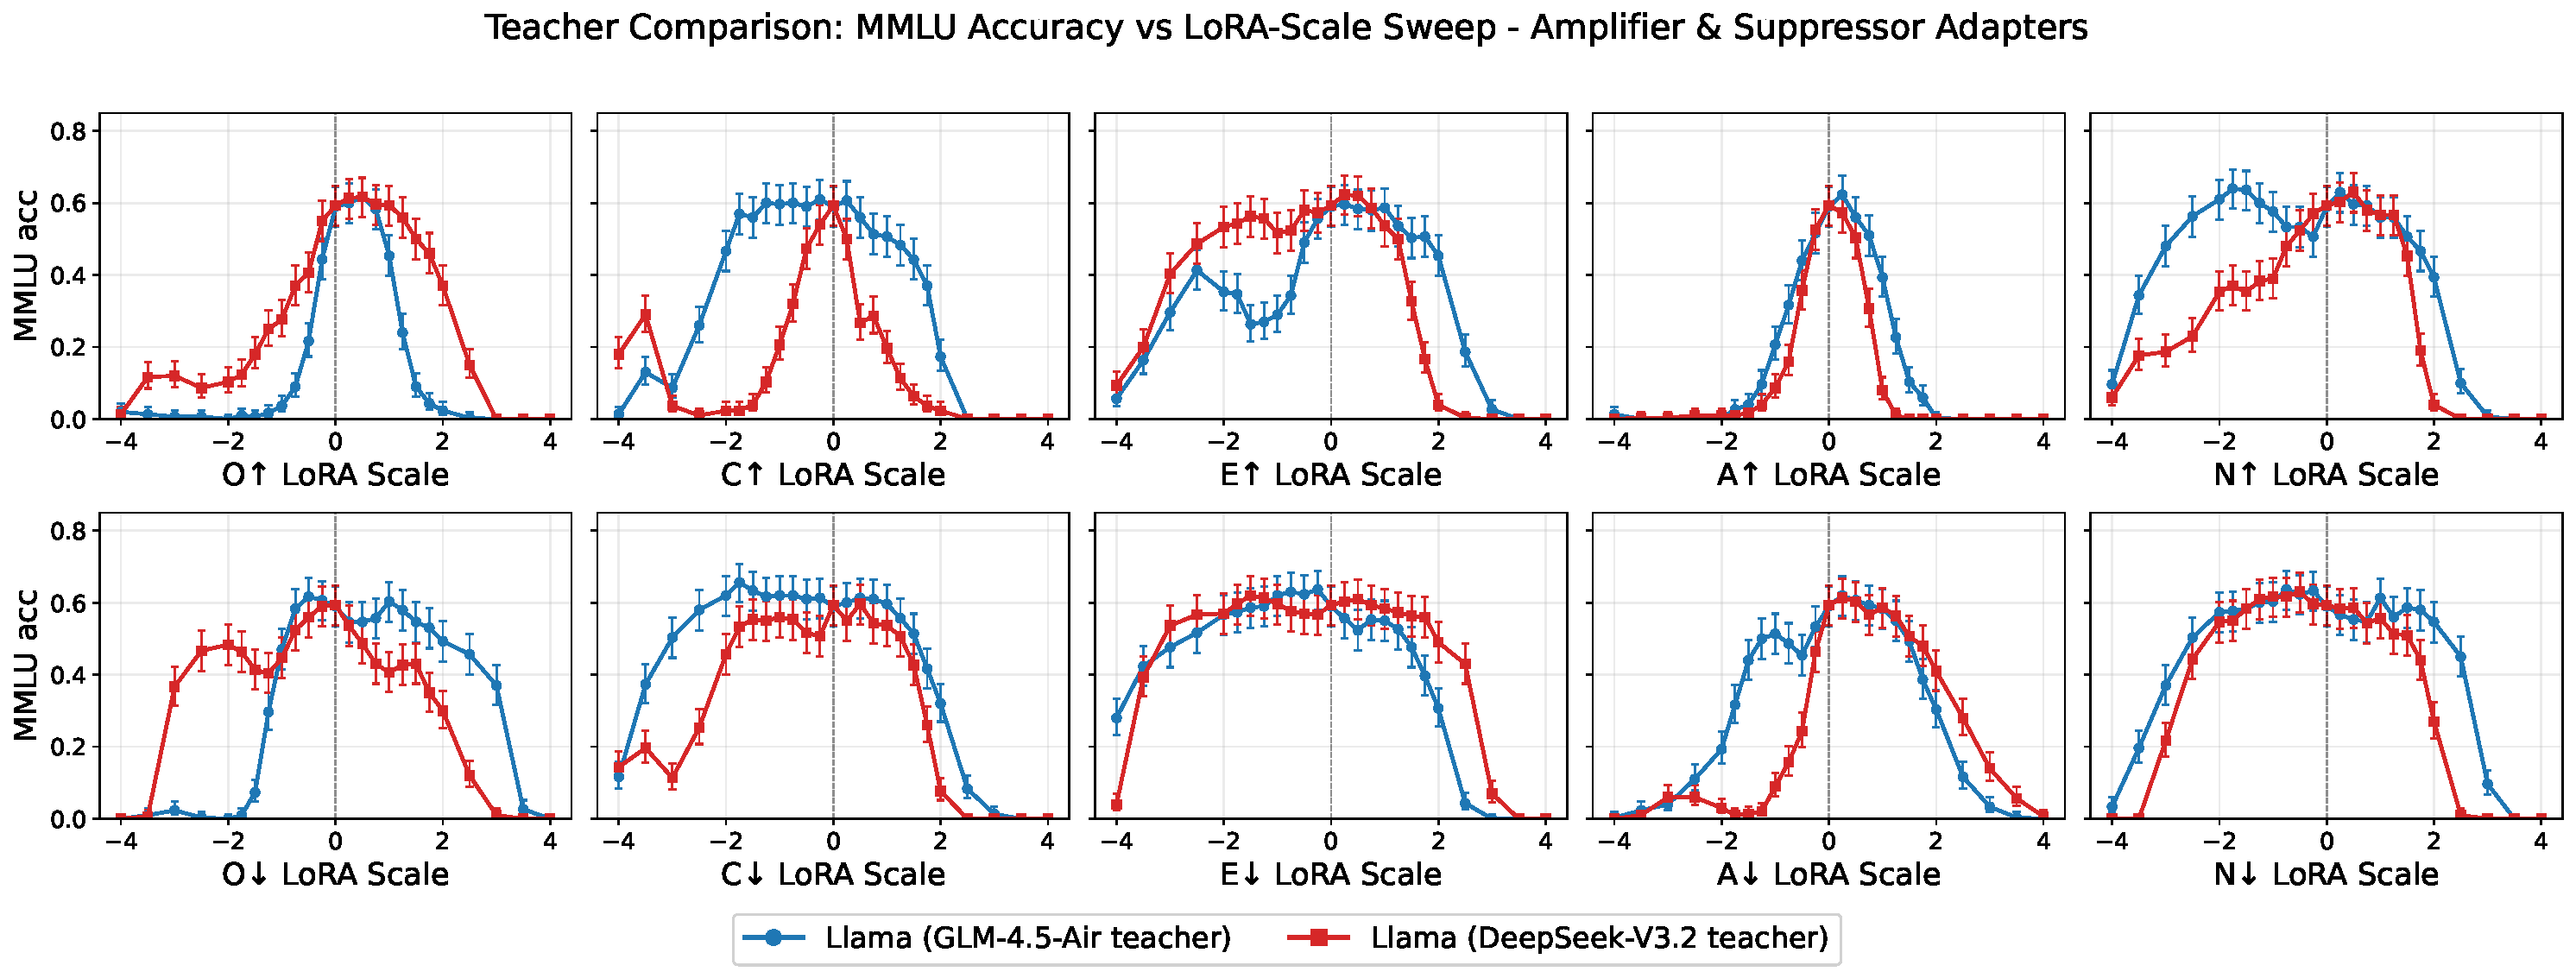
\includegraphics[width=\linewidth]{figures/appendix/model_comparison/fig_teacher_mmlu.pdf}
\caption{\textbf{MMLU capability retention across teachers.} Rows: adapter
direction (amplifier / suppressor); columns: applied OCEAN adapter. MMLU accuracy
vs LoRA scale, one line per teacher.}
\label{fig:teacher-mmlu}
\end{figure}

\begin{figure}[htbp]
\centering
% Generated by: scripts/visualisations/model_comparison_ocean_transfer.py --set llama_teacher
% Data: HF persona-shattering-lasr/monorepo @ fine_tuning/llama-3.1-8b-it/other/ocean_def_control/amplifier/{ocean_const_paired_dpo_s1vs2, ocean_const_paired_dpo_teacher_dsv32_s1vs2}/evals/mcq/mmlu/ — see paper/figures/MANIFEST.md
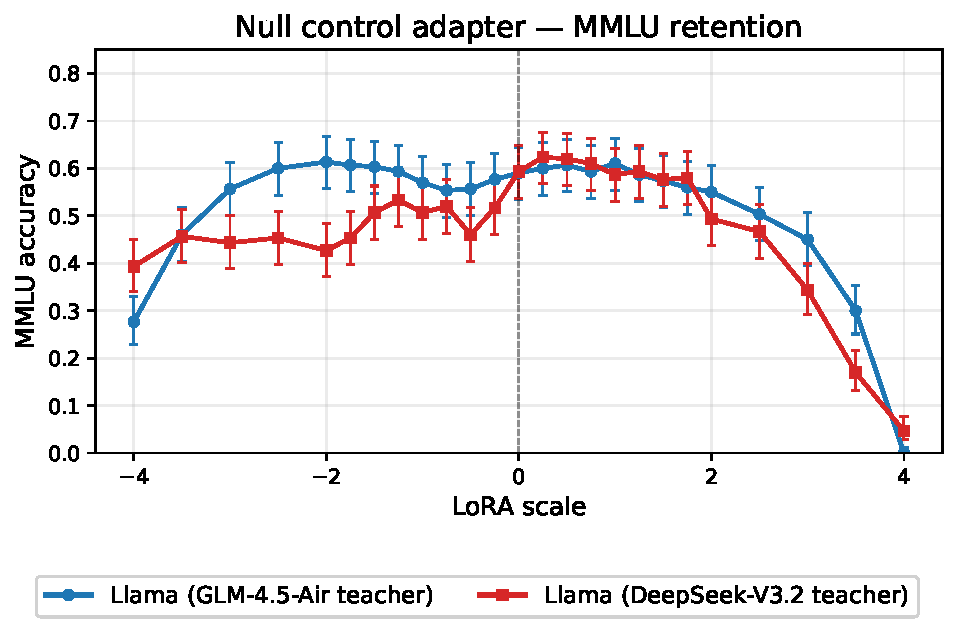
\includegraphics[width=0.6\linewidth]{figures/appendix/model_comparison/fig_teacher_mmlu_control.pdf}
\caption{\textbf{Null control adapter MMLU retention across teachers.} The control
adapter's MMLU accuracy vs LoRA scale, for each teacher.}
\label{fig:teacher-mmlu-control}
\end{figure}

\FloatBarrier
